\chapter{Introduction}
\label{ch:intro}

Dharma is a robot-agnostic autonomy stack for legged and wheeled service robots on ROS~2
Foxy, Humble and Jazzy. It provides LiDAR-inertial odometry with a start gate and a monitor,
fiducial-anchored localization with an extended Kalman filter, occupancy mapping and sites,
route teaching, path planning and following with avoidance around people, a control
multiplexer with a protective field and a latched e-stop, health monitoring, RViz panels and a
simulator. It contains no product features: points of interest, tours, narration and visitor
tracking belong to products built on it (for example the Molly tour-guide robot).

This manual describes version \DharmaVersion. It is written for three readers:
\begin{itemize}
  \item \textbf{integrators} who bring Dharma up on a new robot: Chapters~\ref{ch:arch}
    and~\ref{ch:config} (architecture, robot profile and parameters), Chapter~\ref{ch:control}
    (the safety case) and the interfaces reference (Chapter~\ref{ch:interfaces});
  \item \textbf{developers} who change or extend a package: the subsystem chapters
    (\ref{ch:odometry}--\ref{ch:sim}) with their models and parameters, and
    Chapter~\ref{ch:dev} (layout, style, tests, CI, releases);
  \item \textbf{reviewers} who check that known defects are fixed: Appendix~\ref{app:trace}
    maps every review finding to its fix and its regression test.
\end{itemize}

\section{What changed in 0.2.0}

Version 0.2.0 is a breaking clean-up of the 0.1 stack split out of a product. Two reviews
modelled every subsystem and listed defects with priorities (P0 safety, P1 robustness, P2
maintainability). The main changes:
\begin{itemize}
  \item \textbf{General only.} Points of interest, tours, narration, gestures, visitor tracking
    and the mission status were removed; goals are poses, sites hold a map, fiducials and
    routes.
  \item \textbf{One robot description.} Footprint, base height, kinematics, limits and frames
    come from the shared \param{robot.*} parameters (\code{RobotProfile}); no package declares
    its own geometry.
  \item \textbf{Structure.} Every package has a pure \code{core/} (no ROS imports), a
    \code{utils/} with conversions and thin nodes on \code{DharmaNode}; modules have at most
    300 lines; families of algorithms are plugins.
  \item \textbf{Typed interfaces.} Status topics are typed messages with enum constants;
    safety actions are separate trigger services.
  \item \textbf{Safety.} One braking model for every speed limit; the protective field covers
    rotation and combined motion; blind or stale sensing is an obstacle; the e-stop latches
    reasons, has a hardware input and requires a re-arm; navigation never publishes the
    robot's \topic{cmd_vel}.
  \item \textbf{Estimation.} Gravity-aligned odometry, an EKF over \frm{map}$\to$\frm{odom} with
    covariance and chi-square gating, optional scan matching, mapping with jump and correction
    gates.
\end{itemize}

\section{Conventions of this manual}

Frames, topics, services and parameters are set in \code{typewriter}. Topic names are
relative: a product namespaces the robot driver (\code{/<ns>/cmd_vel}). Units are SI; angles
are radians internally and degrees only in human-facing configuration (parameter names end in
\code{_deg}). A transform $\T{a}{b}$ is the pose of frame $b$ in frame $a$, i.e.\ the TF edge
$a \to b$; it maps points from $b$ to $a$. This edition describes the 0.2.0 code of every
repository; the parameter and interface tables are generated from it
(\code{docs/manual/tools/reference.py}). Measured results are reported in the paper, not here.

\section{Repositories}

\begin{figure}[h]
  \centering
  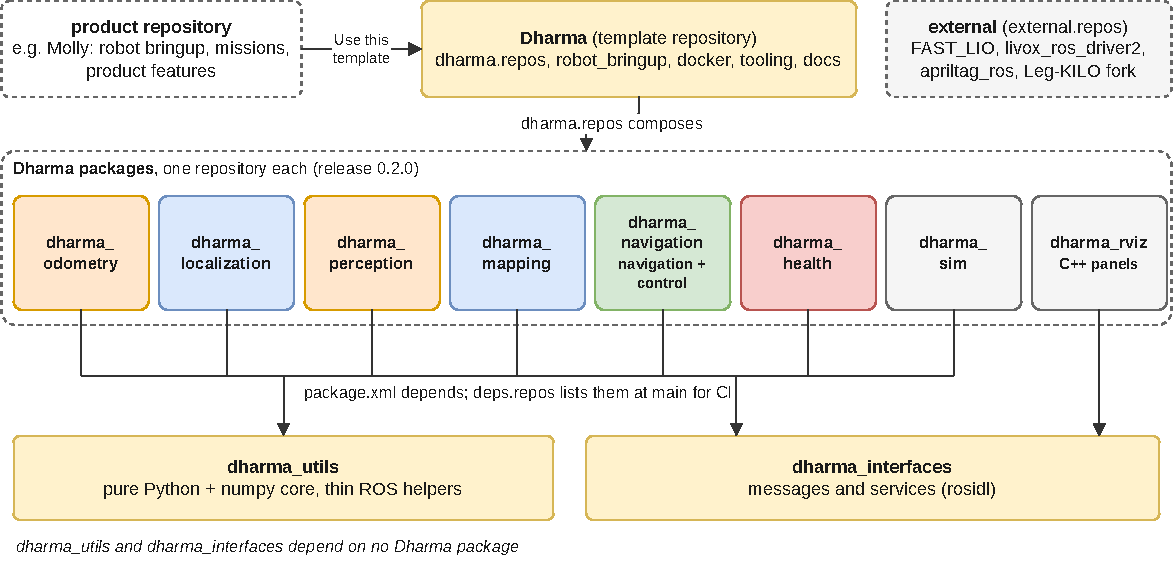
\includegraphics[width=\textwidth]{repos}
  \caption{Repositories and their dependencies. Every package depends only on
    \pkg{dharma_utils} and \pkg{dharma_interfaces}; the Dharma template repository composes
    them, and a product is generated from the template.}
  \label{fig:repos}
\end{figure}

\begin{tabularx}{\textwidth}{@{}lX@{}}
  \toprule
  Repository & Content \\
  \midrule
  \pkg{dharma_utils} & math, typed configuration, robot profile, braking model, io, grid, plugins,
    logging, ROS node helpers, test helpers \\
  \pkg{dharma_interfaces} & messages and services \\
  \pkg{dharma_odometry} & estimator launch (FAST-LIO2, Leg-KILO or external), start gate, monitor \\
  \pkg{dharma_localization} & bridge, EKF over \frm{map}$\to$\frm{odom}, fiducial tags \\
  \pkg{dharma_perception} & sector and safety scans from the LiDAR, camera throttle for fiducials \\
  \pkg{dharma_mapping} & occupancy grid, sites, route recorder \\
  \pkg{dharma_navigation} & packages \pkg{dharma_navigation} (planner, loader, follower,
    avoidance) and \pkg{dharma_control} (control mux) \\
  \pkg{dharma_health} & health monitor and diagnostics \\
  \pkg{dharma_rviz} & RViz panels (C++) \\
  \pkg{dharma_sim} & simulator with drift, latency and dropout \\
  \code{Dharma} & template repository: workspace, docker, bringup skeleton, tooling, documentation \\
  \bottomrule
\end{tabularx}
